\documentclass[12pt,twoside]{book}
\usepackage{layout}
%\usepackage{makeidx}
\RequirePackage{verbatim}
%\RequirePackage{alltt}
\usepackage{ifpdf}
\usepackage{etoolbox}
\usepackage{mathtools}


\newtoggle{solutions}
\toggletrue{solutions}
\togglefalse{solutions}

\ifpdf 
   \pdfcompresslevel=9
   \pdfoutput=1
                                                                                            
                       
   \usepackage[pdftex]{graphicx}
   \usepackage[pdftex]{geometry}
   \usepackage[pdftex]{color}
   \usepackage{hyperref}
   \hypersetup{
     pdftitle={Recitation Activities for the Introduction to Differential Equations},
     pdfsubject={ODE},
     pdfauthor={Kelly Black},
     pdfkeywords={classroom activities},
     anchorcolor = {red},
     colorlinks = {true},
     %pdfpagemode={FullScreen}
   }
\else
   \usepackage{epsfig}
   \usepackage{color}
\fi
\usepackage[table]{xcolor}


\pagestyle{myheadings}

%\setlength{\basicoddside}{\oddsidemargin}
%\setlength{\basicevenside}{\evensidemargin}
%\setlength{\basicwidth}{\textwidth}
%\setlength{\basictop}{\topmargin}
%\setlength{\basicheight}{\textheight}


\newcommand{\introduction}[1]{}

\font\tenit=cmti10
\makeatletter

\renewcommand{\@evenfoot}{\tenit Clarkson University Division of
  Mathematics and Computer Science \hfill}
\renewcommand{\@oddfoot}{\tenit \hfill Math 232: Introduction to
  Differential Equations - \today}

\renewcommand{\section}{\@startsection
  {section}
  {1}
  {0em}
  {\baselineskip}
  {-1em}
  {\normalfont\normalsize\bfseries}}

\renewcommand{\subsection}{\@startsection
  {subsection}
  {2}
  {0em}
  {\baselineskip}
  {-1em}
  {\normalfont\normalsize\bfseries}}

\renewcommand{\subsubsection}{\@startsection
  {subsubsection}
  {2}
  {0em}
  {\baselineskip}
  {-2em}
  {\normalfont\normalsize\itshape}}

\makeatother


\newlength{\basicoddside}
\newlength{\basicevenside}
\newlength{\basicwidth}
\newlength{\basictop}
\newlength{\basicheight}

\newcommand{\activityParams}{
  %\setlength{\hoffset}{0in}
  %\setlength{\oddsidemargin}{-0.5in}
  %\setlength{\evensidemargin}{-0.5in}
  %\setlength{\textwidth}{7.5in}
  \setlength{\topmargin}{-0.5in}
  \setlength{\textheight}{9in}
}

\newcommand{\textParams}{
  \setlength{\oddsidemargin}{\basicoddside}
  \setlength{\evensidemargin}{\basicevenside}
  \setlength{\textwidth}{\basicwidth}
  \setlength{\topmargin}{\basictop}
  \setlength{\textheight}{\basicheight}
}


  \setlength{\oddsidemargin}{-0.25in}
  \setlength{\evensidemargin}{0.25in}
  \setlength{\textwidth}{6.25in}
  \setlength{\topmargin}{-0.5in}
  \setlength{\textheight}{9in}
  \setlength{\marginparwidth}{56pt}


\newcommand{\sideNote}[1]{\marginpar{\tenit \raggedright #1}}
\newcommand{\doNotPrint}[1]{}


\newtheorem{lemma}{Lemma}[subsection]
\newtheorem{theorem}{Theorem}[subsection]



\newcounter{activity}
\setcounter{activity}{1}

\newcommand{\actTitle}[1]{
  \cleardoublepage
  \activityParams
  \stepcounter{activity}
  \markboth
  {Name: \hspace*{2.5in} \hfil  Activity: \theactivity}
  {Name: \hspace*{2.5in} \hfil  Activity: \theactivity}
  \stepcounter{subsection}
  \addcontentsline{toc}{subsection}{
    \protect\numberline{\thesubsection}{#1}}
}

\newcounter{hw}
\setcounter{hw}{0}
\newcommand{\hwTitle}[1]{
  \cleardoublepage
  \activityParams
  \stepcounter{hw}
  \markboth
  {Name: \hspace*{2.5in} \hfil  Home Work: \thehw}
  {Name: \hspace*{2.5in} \hfil  Home Work: \thehw}
  \stepcounter{subsubsection}
  \addcontentsline{toc}{subsubsection}{
    \protect\numberline{\thesubsubsection}{#1}}
}

\newcommand{\preClass}[1]{
  \cleardoublepage
  \activityParams
  \markboth
  {Name: \hspace*{2in} \hfil Preclass Work - Finish Before Class Begins \hfil}
  {Name: \hspace*{2in} \hfil Preclass Work - Finish Before Class Begins \hfil}
  \stepcounter{subsubsection}
  \addcontentsline{toc}{subsubsection}{
    \protect\numberline{\thesubsubsection}{#1}}
}

\newcommand{\postClass}{

  \cleardoublepage
  \activityParams
  \markboth
  {Name: \hspace*{2in} \hfil Postclass Work - Finish After Class \hfil}
  {Name: \hspace*{2in} \hfil Postclass Work - Finish After Class \hfil}
%  \stepcounter{subsubsection}
%  \addcontentsline{toc}{subsubsection}{
%    \protect\numberline{\thesubsubsection}{#1}}
}


\newcounter{quiz}
\setcounter{quiz}{1}
\newcommand{\qzTitle}[1]{
  \cleardoublepage
  \activityParams
  \stepcounter{quiz}
  \markboth
  {Name: \hspace*{2.5in} \hfil  #1 Quiz: \thequiz}
  {Name: \hspace*{2.5in} \hfil  #1 Quiz: \thequiz}
  \stepcounter{subsubsection}
  \addcontentsline{toc}{subsubsection}{
    \protect\numberline{\thesubsubsection}{#1}}
}


\newcommand{\stateSummary}{\item State and summarize two ideas from today's
  class. 
  \vfill 
  \centerline{\textit{(Over)}}
  \clearpage }


\newcommand{\addTOC}[1]{
  \stepcounter{section}
  \addcontentsline{toc}{section}{
    \protect\numberline{\thesection}{#1}}
  }



\newenvironment{problem}
{\begin{list}
{\arabic{enumi}.}
{\usecounter{enumi}
\setlength{\rightmargin}{0pt}
%\setlength{\rightmargin}{-72pt}
\setlength{\parsep}{1em}
\setlength{\listparindent}{0pt}
}}
{\end{list}}

\newenvironment{subproblem}
{\begin{list}
{(\alph{enumii})}
{\usecounter{enumii}
\setlength{\rightmargin}{0pt}
\setlength{\parsep}{1em}
\setlength{\listparindent}{0pt}
}}
{\end{list}}

\newenvironment{multiEqn}
{\begin{eqnarray*} 
 \begin{array}{rclclclcl}}
{\end{array}
 \end{eqnarray*}}


\setcounter{activity}{0}



% %%%%%%%%%%%%%%%%%%%%%%%%%%%%%%%%%%%%%%%%%%%%%%%%%%%%%%%%%%%%%%%%%%%%%%%
% List of definitions that are used in the different pages for the
% notes

% %%%%%%%%%%%%%%%%%%%%%%%%%%%%%%%%%%%%%%%%%%%%%%%%%%%%%%%%%%%%%%%%%%%%%%%
% Basic definitions used throughout the notes

\newcommand{\half}{\mbox{$\frac{1}{2}$}}
\newcommand{\deltat}{\mbox{$\triangle t$}}
\newcommand{\deltax}{\mbox{$\triangle x$}}
\newcommand{\deltay}{\mbox{$\triangle y$}}

\newcommand{\deriv}[2]{\frac{d}{d#2}#1}
\newcommand{\derivTwo}[2]{\frac{d^2}{d#2^2}#1}

\newcommand{\lp}{\left(}
\newcommand{\rp}{\right)}

% %%%%%%%%%%%%%%%%%%%%%%%%%%%%%%%%%%%%%%%%%%%%%%%%%%%%%%%%%%%%%%%%%%%%%%
% Basic color additions
\definecolor{fuchsia}{RGB}{255,0.0,255}
\definecolor{garnet}{RGB}{136,0,0}
\definecolor{light-blue}{RGB}{100,100,255}
\definecolor{light-red}{RGB}{255,100,100}
\definecolor{georgiaRed}{RGB}{100,0,00}
\definecolor{light-gray}{gray}{0.8}
\definecolor{mediumGray}{gray}{0.6}
\definecolor{clarksonGreen}{RGB}{0,52,21}


\newcommand{\redText}[1]{{\color{red}#1}}
\newcommand{\blueText}[1]{{\color{blue}#1}}
\newcommand{\fuchsiaText}[1]{{\color{fuchsia}#1}}

%%% Local Variables:
%%% mode: latex
%%% TeX-master: t
%%% End



%\includeonly{laplace}

\begin{document}


\title{Recitation Activities \\ 
  Introduction to Statistics
  \iftoggle{solutions}{%
    \\\textit{Solution Manual}
  }
}
\author{Kelly Black\\Clarkson University\\Division of Mathematics and
  Computer Science}

\maketitle

\textit{\small Inside of front cover - (intentionally blank)
  \tiny{well mostly blank....}}

\clearpage

\begin{center}
  
  
\includegraphics{img/ccV3}

  Recitation Activities for the Introduction to Statistics
  by Kelly Black is licensed under a Creative Commons
  Attribution-NonCommercial-ShareAlike 3.0 Unported License.

  Special thanks go to Khrystyna Dilai and Justin Foster who made the
  first draft of all of the files.

  \url{http://creativecommons.org/licenses/by-nc-sa/3.0/ }

\end{center}


\tableofcontents

%\clearpage

\chapter{Probability}

\documentclass[12pt]{article}

\oddsidemargin=0.0in
\evensidemargin=0.0in
\textwidth=6in
\topmargin=-1in
\textheight=9.5in

\setlength{\parindent}{0pt}

\begin{document}

 \textbf{Probability: Introduction} \\
\\
\textit{You are not expected to finish this during the class period. Anything you don't finish is good to practice at home.}  \\ [5pt]

\textbf{Definition:} \\ [5pt]

 The \textit{probability} of an outcome is the long term proportion in which the outcome is observed. \\
\\
Probabilities reveal long term predictability. \\
\\
If probability = 0, outcome is \textit{impossible}. \\
If probability is = 1, outcome is a \textit{certainty}. \\ 

\textbf{Define the following terms in your own words :} (1 or 2 sentences) \\ [5pt]
Event:\\  [12pt]
Outcome: \\ [12pt]
Experiment:\\ [12pt]
Observational Study: \\ [12pt]
Expected Outcome:\\ [12pt]
Variation:\\

 \textbf{Experiment :}

 Flip a coin 10 times and record the total sample proportion of heads each time, including the previous flips.\\

\begin{tabular}{| c | c | r |}
 \hline 
Number of Flips & Number of Heads & Sample Proportion of Heads \\  \hline 
1 &  & \\  [12pt] \hline 
2 & & \\  [12pt]  \hline 
3 & & \\ [12pt]  \hline 
4 & & \\  [12pt]  \hline 
5 & & \\  [12pt]  \hline 
\end{tabular}  
\\
Find a partner and put your data together. Describe what happens to the proportion when you have 10 flips? 20 flips? More?\\
\vspace{5em}
\\

Make a bar graph of the total frequency of heads and tails for 20 flips. \\
\vspace{10em}

\textbf{Definititon:}\\

\textit{Sample space:}  is the collection of all possible \textit{events}. \\

\textit{Venn Diagrams} and \textit{ Tree Diagrams} are ways to visualize sample space.
\\

\textbf{Practice:}

\begin{enumerate}
\item You flip a fair coin. Define the sample space of this experiment by writing down all the possible events.\\

\begin{itemize}
 \item Repeat the exercise again but for flipping a coin 2 times?\\
 \vspace{2em}
 
 \item How about 3 times? Draw a tree diagram to represent all possible events when you flip a coin 3 times.\\
\vspace{7em}

  \end{itemize}
  
\item In a class of 30 students, 10 chose \textbf{only} art as an elective, 2 chose both, 14 chose music. How many chose neither?
\textit{Draw the sample space using an appropriate diagram.}\\ 
\vspace{5em}

 \end{enumerate}

\clearpage

\textbf{Application:} \textit{This activity will be done as a class.} \\ [12pt]

A volunteer will pick beans out of a bag. Every time a bean is picked, record the total number of black beans picked in the middle column. (Include previous trials.) In the right column record the total sample proportion of black beans picked every time you pick another bean. \\

\begin{tabular}{| c | c | r |}
 \hline 
Number & Number of Black & Proportion of Black \\  \hline 
1 &  & \\  [12pt] \hline 
2 & & \\  [12pt] \hline 
3 & & \\  [12pt] \hline 
4 & & \\  [12pt]  \hline 
5 & & \\  [12pt] \hline 
6 & & \\  [12pt] \hline 
7 & & \\  [12pt] \hline 
8 & & \\  [12pt] \hline 
9 & & \\  [12pt] \hline 
10 & & \\  [12pt] \hline 
\end{tabular}
\\
\\
Based on the results what is the predicted proportion of black beans? \\


 
 \clearpage
 
\textbf{Define the following terms in your own words:} (1-2 sentences) \\

\textit{Mutually exclusive/disjoint}: \\[12pt] 
\textit{Addition rule:} \\ [12pt] 
\textit{Complement Rule:} \\ [12pt] 
\textit{Multiplication Rule:} \\ [12pt] 
\textit{Conditional Probabilities:}  \\ [12pt] 

\textbf{Examples:}\\

\begin{enumerate}

\item What is the probability of drawing a king or a queen from a standard 52 card deck?\\   % Addition
\vspace{2em}

\item What is the probability of rolling a 1 or a  6 on a standard six sided die?\\   % Addition
\vspace{2em}

\item The probability of \textit{S} is 0.6, the probability of \textit{Y} is 0.4 the probability of \textit{S} and \textit{Y} is 0.5. What is the probability of \textit{S} or \textit{Y}?. \\  
\vspace{2em}

\item What is the probability of picking a queen or a heart ?\\ %Addition
\vspace{2em}

\item What is the probability of not rolling a 6 or rolling a 1 on a standard 6 sided die ? \\ % Addition
\vspace{2em}

\item What is the probability of getting 3 heads when flipping a coin?\\  % Multiplication 
\vspace{2em}

\item What is the probability of getting a H T H when flipping a coin? \\ % Multiplication
\vspace{2em}

\item What is the probability that an outcome of rolling a standard six sided die is 4 given that the number is even?\\ %Conditional 
\vspace{2em}

\item What is the probability of picking a queen out a deck of cards given that the card is red?\\ %Conditional 
\vspace{2em}

\item What is the probability of drawing a king followed by a queen from a standard 52 card deck without replacement?\\   % Multiplication
\vspace{2em}

\item You roll a die twice. What is the probability of getting exactly one 1. \\  % Addition and Multilication
\vspace{2em}

\item What is the probability of picking a queen followed by not a heart without replacement ?\\  % Multiplication and Addition
\vspace{2em}

\item What is the probability of rolling at least a 4 on a standard six sided die?\\  % Addition 
\vspace{2em}

\end{enumerate}



\end{document}




      % 1, 2, 3 and 4
\documentclass[12pt]{article}

\oddsidemargin=0.0in
\evensidemargin=0.0in
\textwidth=6in
\topmargin=-1in
\textheight=9.5in

\setlength{\parindent}{0pt}

\begin{document}

 \textbf{Probability: Counting} \\
\\
\textit{You are not expected to finish this during the class period. Anything you don't finish is good to practice at home.}  \\ [5pt]

\textbf{Please define the following terms in your own words:} (1 or 2 sentences) \\ [5pt]

  \textit{Probability:} \\
\\
\textit{Certain vs. Impossible}\\

\textbf{Definittions:}  \\ [5pt]
\textit{Counting: } Determining the number of outcomes that sequence of events could result in.  Ex: There are 3 types of cones in an ice cream store and 10 flavors therefore there are 30 different types of cone and ice cream combinations if only one cone and one flavor is chosen.\\  [12pt]

\textit{Factorial: }Used to represent the number of ways that k number of objects can be ordered. k! = k x (k-1) x (k-2) x ... x 1.  Remember 0! = 1. \\ [12pt]


 \textbf{Examples:}

\begin{enumerate}
\item In how many different ways can a cross country race be completed if there are 5 runners and no ties?\\

\item If a multiple choice test has 10 questions with 5 choices for each questions in how many different ways can you complete the test?\\

\item A license plate has three letters and 3 digits. How many different license plates can be made made? \\

\item An ID number begins with a letter and is followed by 4 numbers. How many different ID numbers can be made? \\
\end{enumerate}

\textbf{Definititon:}\\

\textit{Permutation:}   An ordering of a set of distinct objects.  \\  [12pt]
Notation: nPr where \textit{n} is the number of distinct objects and \tectit{r} is the number of objects taken at a time.  Order matters.\\[12pt]
Example: How many different can this set of letters be arranged if two letters are used in a group?\\[12pt]
Letter Set: ABC\\[12pt]
Possible permutations: AA, AB,  AC, BA,  BB,  BC, CA, CB,  CC\\ [12pt]

\textit{Combination:}  A combination of a a number of elements form a set where order does not matter. \\ [12pt]
Example: How many different combinations of 2 letters can be made from these 3 letters?\\ [12pt]
Letter Set: ABC\\ [12pt]
Possible combinations: AB,  AC,  BA, BC, CA, CB. \\ [12pt]

\textbf{Formulas:}

Write the formula for perambulations: \\

Write the formula for combinations: \\

\textbf{Practice:}



\begin{enumerate}


\end{document}




          % 5 and 6
\documentclass[12pt]{article}

\oddsidemargin=0.0in
\evensidemargin=0.0in
\textwidth=6in
\topmargin=-1in
\textheight=9.5in

\setlength{\parindent}{0pt}

\begin{document}

 \textbf{Probability: Discrete Random Variables} \\
\\
\textit{You are not expected to finish this during the class period. Anything you don't finish is good to practice at home.}  \\ [5pt]

\textbf{Please define the following terms in your own words:} (1 or 2 sentences) \\ [5pt]

 \textit{Random Variable:} \\
\\
\textit{Discrete Random Variable:}\\


\textbf{Definittions:}  \\ [5pt]

\textit{Probability Mass Function: } (PMF) The probability that a discrete random variable is exactly equal to some value.  A PMF is equal to values between 0 and 1 with the sum of those values adding up to 1. \\  [12pt]

How would you graph a probability mass function? \\ [12pt]


 \textbf{Examples: } \\

\begin{enumerate}

\item List three examples of discrete random variables.\\[12pt]


\item Toss a coin and let Y equal the number of tails. Find the PMF of Y. \\[12pt]


\item Toss a coin twice and let Y equal the number of tails. Find the PMF of Y.\\[12pt]


\item You toss two six sided fair dice. The number of miles you have to run is equal to the sun on the dice and Y is equal to the number of miles you have to run after tossing the dice once. Find and graph the PMF of Y. \\[12pt]



\end{enumerate}

\end{document}




      % 7 and 8

\preClass{Counting}


\begin{problem}
\item Examples of uniform probability distributions.

  \begin{subproblem}
  \item 
    \begin{eqnarray}
      y & = 3x + 4.
    \end{eqnarray}
    \vfill
  \end{subproblem}


\end{problem}


\actTitle{Uniform and Normal Distribution} 

\begin{problem}

\item The flexibility of a patient's knee extension is evaluated as
  the angle that a patient can rotate her knee and is measured with a
  goniometer. It is estimated that patients who have had a certain
  procedure have a range of angles that is uniformly distributed
  between 10 degrees and 90 degrees.

  \begin{subproblem}
    \item Sketch a plot of the distribution. (Label and mark your
      axes!).

      \vfill

    \item On your plot shade in the are associated with the people
      who can move their knee to an angle of 40 degrees or less.
      
    \item A patient who has had the procedure is chosen at
      random. What is the probability that the person will be able to
      move their knee through an angle of 40 degrees or less?

      \vspace{2em}

    \item A patient who has had the procedure is chosen at
      random. What is the probability that the person will be able to
      move their knee through an angle of 40 degrees or more?

      \vspace{2em}

    \item A patient who has had the procedure is chosen at
      random. What is the probability that the person will be able to
      move their knee through an angle of 50 degrees to 60 degrees?

      \vfill


  \end{subproblem}

\clearpage

\item Sketch a plot of a normal distribution that has a mean of 3.0
  and a standard deviation of 1.0. Shade in the area associated with
  the values less than or equal to 1.5. (Label and mark your axes!)

  \vfill

\item Financial analysts who make forecasts are categorized as either
  being ``buy-side'' or ``sell-side'' analysts. It is estimated that
  the forecast error for buy-side analysts is 0.85 with a standard
  deviation of 1.93. It is estimated that the forecast error for
  sell-side analysts is -0.05 with a standard deviation of
  0.85. Sketch plots for the distributions for the two types of
  analysts assuming the errors are normally distributed. For each
  distribution shade in the area associated with errors greater than
  1.1 or less than -1.1. (Label and mark your axes!)

  \vfill
  
\end{problem}


\actTitle{The Standard Normal Distribution} 


Approximation of the cumulative distribution for the standard normal distribution. 
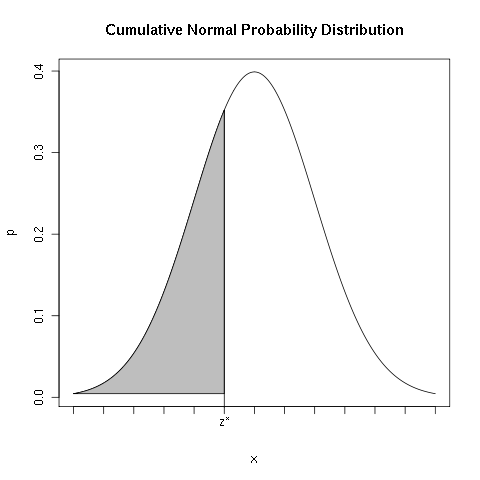
\includegraphics[height=3.25cm]{img/cummulativeDist}

\begin{tabular}{l|llllllllll}
     & 0.00   & 0.01   & 0.02   & 0.03   & 0.04   & 0.05   & 0.06   & 0.07   & 0.08  & 0.09 \\ \hline
-3.4 & 0.0003 & 0.0003 & 0.0003 & 0.0003 & 0.0003 & 0.0003 & 0.0003 & 0.0003 & 0.0003 & 0.0002 \\\arrayrulecolor{light-gray}\hline\arrayrulecolor{black} 
-3.3 & 0.0005 & 0.0005 & 0.0005 & 0.0004 & 0.0004 & 0.0004 & 0.0004 & 0.0004 & 0.0004 & 0.0003 \\\arrayrulecolor{light-gray}\hline\arrayrulecolor{black} 
-3.2 & 0.0007 & 0.0007 & 0.0006 & 0.0006 & 0.0006 & 0.0006 & 0.0006 & 0.0005 & 0.0005 & 0.0005 \\\arrayrulecolor{light-gray}\hline\arrayrulecolor{black} 
-3.1 & 0.0010 & 0.0009 & 0.0009 & 0.0009 & 0.0008 & 0.0008 & 0.0008 & 0.0008 & 0.0007 & 0.0007 \\\arrayrulecolor{light-gray}\hline\arrayrulecolor{black} 
-3.0 & 0.0013 & 0.0013 & 0.0013 & 0.0012 & 0.0012 & 0.0011 & 0.0011 & 0.0011 & 0.0010 & 0.0010 \\\arrayrulecolor{light-gray}\hline\arrayrulecolor{black} 
-2.9 & 0.0019 & 0.0018 & 0.0018 & 0.0017 & 0.0016 & 0.0016 & 0.0015 & 0.0015 & 0.0014 & 0.0014 \\\arrayrulecolor{light-gray}\hline\arrayrulecolor{black} 
-2.8 & 0.0026 & 0.0025 & 0.0024 & 0.0023 & 0.0023 & 0.0022 & 0.0021 & 0.0021 & 0.0020 & 0.0019 \\\arrayrulecolor{light-gray}\hline\arrayrulecolor{black} 
-2.7 & 0.0035 & 0.0034 & 0.0033 & 0.0032 & 0.0031 & 0.0030 & 0.0029 & 0.0028 & 0.0027 & 0.0026 \\\arrayrulecolor{light-gray}\hline\arrayrulecolor{black} 
-2.6 & 0.0047 & 0.0045 & 0.0044 & 0.0043 & 0.0041 & 0.0040 & 0.0039 & 0.0038 & 0.0037 & 0.0036 \\\arrayrulecolor{light-gray}\hline\arrayrulecolor{black} 
-2.5 & 0.0062 & 0.0060 & 0.0059 & 0.0057 & 0.0055 & 0.0054 & 0.0052 & 0.0051 & 0.0049 & 0.0048 \\\arrayrulecolor{light-gray}\hline\arrayrulecolor{black} 
-2.4 & 0.0082 & 0.0080 & 0.0078 & 0.0075 & 0.0073 & 0.0071 & 0.0069 & 0.0068 & 0.0066 & 0.0064 \\\arrayrulecolor{light-gray}\hline\arrayrulecolor{black} 
-2.3 & 0.0107 & 0.0104 & 0.0102 & 0.0099 & 0.0096 & 0.0094 & 0.0091 & 0.0089 & 0.0087 & 0.0084 \\\arrayrulecolor{light-gray}\hline\arrayrulecolor{black} 
-2.2 & 0.0139 & 0.0136 & 0.0132 & 0.0129 & 0.0125 & 0.0122 & 0.0119 & 0.0116 & 0.0113 & 0.0110 \\\arrayrulecolor{light-gray}\hline\arrayrulecolor{black} 
-2.1 & 0.0179 & 0.0174 & 0.0170 & 0.0166 & 0.0162 & 0.0158 & 0.0154 & 0.0150 & 0.0146 & 0.0143 \\\arrayrulecolor{light-gray}\hline\arrayrulecolor{black} 
-2.0 & 0.0228 & 0.0222 & 0.0217 & 0.0212 & 0.0207 & 0.0202 & 0.0197 & 0.0192 & 0.0188 & 0.0183 \\\arrayrulecolor{light-gray}\hline\arrayrulecolor{black} 
-1.9 & 0.0287 & 0.0281 & 0.0274 & 0.0268 & 0.0262 & 0.0256 & 0.0250 & 0.0244 & 0.0239 & 0.0233 \\\arrayrulecolor{light-gray}\hline\arrayrulecolor{black} 
-1.8 & 0.0359 & 0.0351 & 0.0344 & 0.0336 & 0.0329 & 0.0322 & 0.0314 & 0.0307 & 0.0301 & 0.0294 \\\arrayrulecolor{light-gray}\hline\arrayrulecolor{black} 
-1.7 & 0.0446 & 0.0436 & 0.0427 & 0.0418 & 0.0409 & 0.0401 & 0.0392 & 0.0384 & 0.0375 & 0.0367 \\\arrayrulecolor{light-gray}\hline\arrayrulecolor{black} 
-1.6 & 0.0548 & 0.0537 & 0.0526 & 0.0516 & 0.0505 & 0.0495 & 0.0485 & 0.0475 & 0.0465 & 0.0455 \\\arrayrulecolor{light-gray}\hline\arrayrulecolor{black} 
-1.5 & 0.0668 & 0.0655 & 0.0643 & 0.0630 & 0.0618 & 0.0606 & 0.0594 & 0.0582 & 0.0571 & 0.0559 \\\arrayrulecolor{light-gray}\hline\arrayrulecolor{black} 
-1.4 & 0.0808 & 0.0793 & 0.0778 & 0.0764 & 0.0749 & 0.0735 & 0.0721 & 0.0708 & 0.0694 & 0.0681 \\\arrayrulecolor{light-gray}\hline\arrayrulecolor{black} 
-1.3 & 0.0968 & 0.0951 & 0.0934 & 0.0918 & 0.0901 & 0.0885 & 0.0869 & 0.0853 & 0.0838 & 0.0823 \\\arrayrulecolor{light-gray}\hline\arrayrulecolor{black} 
-1.2 & 0.1151 & 0.1131 & 0.1112 & 0.1093 & 0.1075 & 0.1056 & 0.1038 & 0.1020 & 0.1003 & 0.0985 \\\arrayrulecolor{light-gray}\hline\arrayrulecolor{black} 
-1.1 & 0.1357 & 0.1335 & 0.1314 & 0.1292 & 0.1271 & 0.1251 & 0.1230 & 0.1210 & 0.1190 & 0.1170 \\\arrayrulecolor{light-gray}\hline\arrayrulecolor{black} 
-1.0 & 0.1587 & 0.1562 & 0.1539 & 0.1515 & 0.1492 & 0.1469 & 0.1446 & 0.1423 & 0.1401 & 0.1379 \\\arrayrulecolor{light-gray}\hline\arrayrulecolor{black} 
-0.9 & 0.1841 & 0.1814 & 0.1788 & 0.1762 & 0.1736 & 0.1711 & 0.1685 & 0.1660 & 0.1635 & 0.1611 \\\arrayrulecolor{light-gray}\hline\arrayrulecolor{black} 
-0.8 & 0.2119 & 0.2090 & 0.2061 & 0.2033 & 0.2005 & 0.1977 & 0.1949 & 0.1922 & 0.1894 & 0.1867 \\\arrayrulecolor{light-gray}\hline\arrayrulecolor{black} 
-0.7 & 0.2420 & 0.2389 & 0.2358 & 0.2327 & 0.2296 & 0.2266 & 0.2236 & 0.2206 & 0.2177 & 0.2148 \\\arrayrulecolor{light-gray}\hline\arrayrulecolor{black} 
-0.6 & 0.2743 & 0.2709 & 0.2676 & 0.2643 & 0.2611 & 0.2578 & 0.2546 & 0.2514 & 0.2483 & 0.2451 \\\arrayrulecolor{light-gray}\hline\arrayrulecolor{black} 
-0.5 & 0.3085 & 0.3050 & 0.3015 & 0.2981 & 0.2946 & 0.2912 & 0.2877 & 0.2843 & 0.2810 & 0.2776 \\\arrayrulecolor{light-gray}\hline\arrayrulecolor{black} 
-0.4 & 0.3446 & 0.3409 & 0.3372 & 0.3336 & 0.3300 & 0.3264 & 0.3228 & 0.3192 & 0.3156 & 0.3121 \\\arrayrulecolor{light-gray}\hline\arrayrulecolor{black} 
-0.3 & 0.3821 & 0.3783 & 0.3745 & 0.3707 & 0.3669 & 0.3632 & 0.3594 & 0.3557 & 0.3520 & 0.3483 \\\arrayrulecolor{light-gray}\hline\arrayrulecolor{black} 
-0.2 & 0.4207 & 0.4168 & 0.4129 & 0.4090 & 0.4052 & 0.4013 & 0.3974 & 0.3936 & 0.3897 & 0.3859 \\\arrayrulecolor{light-gray}\hline\arrayrulecolor{black} 
-0.1 & 0.4602 & 0.4562 & 0.4522 & 0.4483 & 0.4443 & 0.4404 & 0.4364 & 0.4325 & 0.4286 & 0.4247 \\\arrayrulecolor{light-gray}\hline\arrayrulecolor{black} 
-0.0 & 0.5000 & 0.4960 & 0.4920 & 0.4880 & 0.4840 & 0.4801 & 0.4761 & 0.4721 & 0.4681 & 0.4641 \\\arrayrulecolor{light-gray}\hline\arrayrulecolor{black} 
\end{tabular}


\clearpage
 Approximation of the cumulative distribution for the standard normal distribution. 
 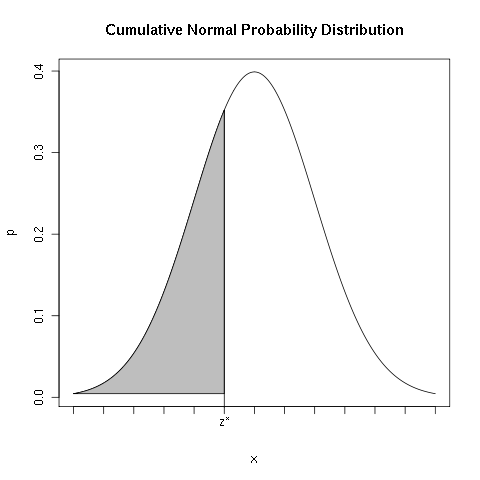
\includegraphics[height=3.25cm]{img/cummulativeDist}

 \begin{tabular}{l|llllllllll}
     & 0.00   & 0.01   & 0.02   & 0.03   & 0.04   & 0.05   & 0.06   & 0.07   & 0.08  & 0.09 \\ \hline
0.0 & 0.5000 & 0.5040 & 0.5080 & 0.5120 & 0.5160 & 0.5199 & 0.5239 & 0.5279 & 0.5319 & 0.5359 \\\arrayrulecolor{light-gray}\hline\arrayrulecolor{black} 
0.1 & 0.5398 & 0.5438 & 0.5478 & 0.5517 & 0.5557 & 0.5596 & 0.5636 & 0.5675 & 0.5714 & 0.5753 \\\arrayrulecolor{light-gray}\hline\arrayrulecolor{black} 
0.2 & 0.5793 & 0.5832 & 0.5871 & 0.5910 & 0.5948 & 0.5987 & 0.6026 & 0.6064 & 0.6103 & 0.6141 \\\arrayrulecolor{light-gray}\hline\arrayrulecolor{black} 
0.3 & 0.6179 & 0.6217 & 0.6255 & 0.6293 & 0.6331 & 0.6368 & 0.6406 & 0.6443 & 0.6480 & 0.6517 \\\arrayrulecolor{light-gray}\hline\arrayrulecolor{black} 
0.4 & 0.6554 & 0.6591 & 0.6628 & 0.6664 & 0.6700 & 0.6736 & 0.6772 & 0.6808 & 0.6844 & 0.6879 \\\arrayrulecolor{light-gray}\hline\arrayrulecolor{black} 
0.5 & 0.6915 & 0.6950 & 0.6985 & 0.7019 & 0.7054 & 0.7088 & 0.7123 & 0.7157 & 0.7190 & 0.7224 \\\arrayrulecolor{light-gray}\hline\arrayrulecolor{black} 
0.6 & 0.7257 & 0.7291 & 0.7324 & 0.7357 & 0.7389 & 0.7422 & 0.7454 & 0.7486 & 0.7517 & 0.7549 \\\arrayrulecolor{light-gray}\hline\arrayrulecolor{black} 
0.7 & 0.7580 & 0.7611 & 0.7642 & 0.7673 & 0.7704 & 0.7734 & 0.7764 & 0.7794 & 0.7823 & 0.7852 \\\arrayrulecolor{light-gray}\hline\arrayrulecolor{black} 
0.8 & 0.7881 & 0.7910 & 0.7939 & 0.7967 & 0.7995 & 0.8023 & 0.8051 & 0.8078 & 0.8106 & 0.8133 \\\arrayrulecolor{light-gray}\hline\arrayrulecolor{black} 
0.9 & 0.8159 & 0.8186 & 0.8212 & 0.8238 & 0.8264 & 0.8289 & 0.8315 & 0.8340 & 0.8365 & 0.8389 \\\arrayrulecolor{light-gray}\hline\arrayrulecolor{black} 
1.0 & 0.8413 & 0.8438 & 0.8461 & 0.8485 & 0.8508 & 0.8531 & 0.8554 & 0.8577 & 0.8599 & 0.8621 \\\arrayrulecolor{light-gray}\hline\arrayrulecolor{black} 
1.1 & 0.8643 & 0.8665 & 0.8686 & 0.8708 & 0.8729 & 0.8749 & 0.8770 & 0.8790 & 0.8810 & 0.8830 \\\arrayrulecolor{light-gray}\hline\arrayrulecolor{black} 
1.2 & 0.8849 & 0.8869 & 0.8888 & 0.8907 & 0.8925 & 0.8944 & 0.8962 & 0.8980 & 0.8997 & 0.9015 \\\arrayrulecolor{light-gray}\hline\arrayrulecolor{black} 
1.3 & 0.9032 & 0.9049 & 0.9066 & 0.9082 & 0.9099 & 0.9115 & 0.9131 & 0.9147 & 0.9162 & 0.9177 \\\arrayrulecolor{light-gray}\hline\arrayrulecolor{black} 
1.4 & 0.9192 & 0.9207 & 0.9222 & 0.9236 & 0.9251 & 0.9265 & 0.9279 & 0.9292 & 0.9306 & 0.9319 \\\arrayrulecolor{light-gray}\hline\arrayrulecolor{black} 
1.5 & 0.9332 & 0.9345 & 0.9357 & 0.9370 & 0.9382 & 0.9394 & 0.9406 & 0.9418 & 0.9429 & 0.9441 \\\arrayrulecolor{light-gray}\hline\arrayrulecolor{black} 
1.6 & 0.9452 & 0.9463 & 0.9474 & 0.9484 & 0.9495 & 0.9505 & 0.9515 & 0.9525 & 0.9535 & 0.9545 \\\arrayrulecolor{light-gray}\hline\arrayrulecolor{black} 
1.7 & 0.9554 & 0.9564 & 0.9573 & 0.9582 & 0.9591 & 0.9599 & 0.9608 & 0.9616 & 0.9625 & 0.9633 \\\arrayrulecolor{light-gray}\hline\arrayrulecolor{black} 
1.8 & 0.9641 & 0.9649 & 0.9656 & 0.9664 & 0.9671 & 0.9678 & 0.9686 & 0.9693 & 0.9699 & 0.9706 \\\arrayrulecolor{light-gray}\hline\arrayrulecolor{black} 
1.9 & 0.9713 & 0.9719 & 0.9726 & 0.9732 & 0.9738 & 0.9744 & 0.9750 & 0.9756 & 0.9761 & 0.9767 \\\arrayrulecolor{light-gray}\hline\arrayrulecolor{black} 
2.0 & 0.9772 & 0.9778 & 0.9783 & 0.9788 & 0.9793 & 0.9798 & 0.9803 & 0.9808 & 0.9812 & 0.9817 \\\arrayrulecolor{light-gray}\hline\arrayrulecolor{black} 
2.1 & 0.9821 & 0.9826 & 0.9830 & 0.9834 & 0.9838 & 0.9842 & 0.9846 & 0.9850 & 0.9854 & 0.9857 \\\arrayrulecolor{light-gray}\hline\arrayrulecolor{black} 
2.2 & 0.9861 & 0.9864 & 0.9868 & 0.9871 & 0.9875 & 0.9878 & 0.9881 & 0.9884 & 0.9887 & 0.9890 \\\arrayrulecolor{light-gray}\hline\arrayrulecolor{black} 
2.3 & 0.9893 & 0.9896 & 0.9898 & 0.9901 & 0.9904 & 0.9906 & 0.9909 & 0.9911 & 0.9913 & 0.9916 \\\arrayrulecolor{light-gray}\hline\arrayrulecolor{black} 
2.4 & 0.9918 & 0.9920 & 0.9922 & 0.9925 & 0.9927 & 0.9929 & 0.9931 & 0.9932 & 0.9934 & 0.9936 \\\arrayrulecolor{light-gray}\hline\arrayrulecolor{black} 
2.5 & 0.9938 & 0.9940 & 0.9941 & 0.9943 & 0.9945 & 0.9946 & 0.9948 & 0.9949 & 0.9951 & 0.9952 \\\arrayrulecolor{light-gray}\hline\arrayrulecolor{black} 
2.6 & 0.9953 & 0.9955 & 0.9956 & 0.9957 & 0.9959 & 0.9960 & 0.9961 & 0.9962 & 0.9963 & 0.9964 \\\arrayrulecolor{light-gray}\hline\arrayrulecolor{black} 
2.7 & 0.9965 & 0.9966 & 0.9967 & 0.9968 & 0.9969 & 0.9970 & 0.9971 & 0.9972 & 0.9973 & 0.9974 \\\arrayrulecolor{light-gray}\hline\arrayrulecolor{black} 
2.8 & 0.9974 & 0.9975 & 0.9976 & 0.9977 & 0.9977 & 0.9978 & 0.9979 & 0.9979 & 0.9980 & 0.9981 \\\arrayrulecolor{light-gray}\hline\arrayrulecolor{black} 
2.9 & 0.9981 & 0.9982 & 0.9982 & 0.9983 & 0.9984 & 0.9984 & 0.9985 & 0.9985 & 0.9986 & 0.9986 \\\arrayrulecolor{light-gray}\hline\arrayrulecolor{black} 
3.0 & 0.9987 & 0.9987 & 0.9987 & 0.9988 & 0.9988 & 0.9989 & 0.9989 & 0.9989 & 0.9990 & 0.9990 \\\arrayrulecolor{light-gray}\hline\arrayrulecolor{black} 
3.1 & 0.9990 & 0.9991 & 0.9991 & 0.9991 & 0.9992 & 0.9992 & 0.9992 & 0.9992 & 0.9993 & 0.9993 \\\arrayrulecolor{light-gray}\hline\arrayrulecolor{black} 
3.2 & 0.9993 & 0.9993 & 0.9994 & 0.9994 & 0.9994 & 0.9994 & 0.9994 & 0.9995 & 0.9995 & 0.9995 \\\arrayrulecolor{light-gray}\hline\arrayrulecolor{black} 
3.3 & 0.9995 & 0.9995 & 0.9995 & 0.9996 & 0.9996 & 0.9996 & 0.9996 & 0.9996 & 0.9996 & 0.9997 \\\arrayrulecolor{light-gray}\hline\arrayrulecolor{black} 
3.4 & 0.9997 & 0.9997 & 0.9997 & 0.9997 & 0.9997 & 0.9997 & 0.9997 & 0.9997 & 0.9997 & 0.9998 \\\arrayrulecolor{light-gray}\hline\arrayrulecolor{black} 
\end{tabular}

\clearpage

\begin{problem}

  \item Find each of the following probabilities for the standard
    normal.
    \begin{subproblem}
      \item $p(Z \leq 0.37)$
        \vfill
      \item $p(Z \leq -0.72)$
        \vfill
      \item $p(Z \leq -2.6)$
        \vfill
      \item $p(Z \leq 0.5)$
        \vfill
      \item $p(Z \geq 0.5)$
        \vfill
      \item $p(Z \leq -0.5)$
        \vfill
      \item $p(Z \geq -0.5)$
        \vfill
      \item $p(Z < 0.5)$
        \vfill
    \end{subproblem}

    \clearpage

  \item Find each of the following probabilities for the standard
    normal.
    \begin{subproblem}
      \item $p((Z \leq 0.37) \mathrm{~and~} (Z \geq -0.37) )$
        \vfill
      \item $p((Z \leq 1.91) \mathrm{~and~} (Z \geq -2.11) )$
        \vfill
      \item $p((Z \leq -2.67) \mathrm{~or~} (Z \geq 2.67) )$
        \vfill
      \item $p((Z \leq -1.17) \mathrm{~or~} (Z \geq 0.71) )$
        \vfill
    \end{subproblem}

  \item For each problem below determine an approximation for $Z_0$
    \begin{subproblem}
      \item $p(Z < Z_0) = 0.05 $
        \vfill
      \item $p(Z < Z_0) = 0.75 $
        \vfill
      \item $p(Z < Z_0) = 0.95 $
        \vfill
      \item $p(Z > Z_0) = 0.25 $
        \vfill
      \item $p(Z > Z_0) = 0.95 $
        \vfill
      \item $p((Z \leq -Z_0) \mathrm{~or~} (Z \geq Z_0) ) = 0.05$
        (Assume that $Z_0>0$.)
        \vfill
      \item $p((Z \geq -Z_0) \mathrm{~and~} (Z \leq Z_0) ) = 0.95$
        (Assume that $Z_0>0$.)
        \vfill
    \end{subproblem}

    \clearpage

\item Financial analysts who make forecasts are categorized as either
  being ``buy-side'' or ``sell-side'' analysts. It is estimated that
  the forecast error for buy-side analysts is 0.85 with a standard
  deviation of 1.93. It is estimated that the forecast error for
  sell-side analysts is -0.05 with a standard deviation of
  0.85. Sketch plots for the distributions for the two types of
  analysts assuming the errors are normally distributed.  Determine
  the following probabilities

  \begin{subproblem}
    \item The probability that a buy-side analyst's error is more than
      1.1.
      \vfill
    \item The probability that a sell-side analyst's error is more than
      1.1.
      \vfill
    \item The probability that a buy-side analyst's error is less than
      -1.1.
      \vfill
    \item The probability that a sell-side analyst's error is less than
      -1.1.
      \vfill
  \end{subproblem}



  
\end{problem}

           % 9 and 10
\preClass{Counting Number of Approaches}


\begin{problem}
\item Examples of uniform probability distributions.

  \begin{subproblem}
  \item 
    \begin{eqnarray}
      y & = 3x + 4.
    \end{eqnarray}
    \vfill
  \end{subproblem}


\end{problem}


\actTitle{Data Collection} 


\begin{problem}

\item An investment bank will conduct a stress test to determine how
  it can react to swings in the markets. As part of the test the
  managers within different offices are asked the following questions:
  \begin{itemize}
  \item What is the total balance in your reserve accounts?
  \item What is the mean error in your return projections over the
    past year?
  \item On a scale from one to five how would you rate your current
    risk? (One means low risk and five is high risk.)
  \item On a scale from one to five how would you rate your current
    operating process? (One means inefficient and five is highly
    efficient.)
  \item When evaluating a fund which aspects of the fund are most
    important in terms of deciding your investment levels? (Circle all
    that apply: \\
    Price; Derivatives; Credit Scoring; Financial Activity; Open
    Options; Dynamic Financial Analysis Projections.
  \end{itemize}

  For each question above determine the nature of the data that will
  result from the survey. Determine if it qualitative, quantitative,
  and if it is quantitative determine if it is ordinal or continuous
  data.

  \vfill

  \clearpage

\item The human resources department examines applications for
  employment. Each applicant answers a number of questions:

  \begin{itemize}
  \item What is your gender? 
  \item What is your age?
  \item What is your racial background?
  \item What is your GPA?
  \item What is your total number of credit hours completed?
  \item What is your expected salary?
  \end{itemize}

  For each question above determine the nature of the data that will
  result from the survey. Determine if it qualitative, quantitative,
  and if it is quantitative determine if it is ordinal or continuous
  data.

  \vfill

  \clearpage

\item Firms that are in bankruptcy are randomly sampled. For each firm
  the reorganization plan in place and the time they have been in
  bankruptcy (in months) is recorded. The data is given below:

  \begin{tabular}{ll|ll|ll} % @{\hspace{3em}
    Plan & Time  (months) & 
    Plan & Time  (months) & 
    Plan & Time  (months)\\ \hline
    None    & 10.1 & Prepack & 4.7  & Prepack & 7.3 \\
    Prepack & 6.7  & Prepack & 7    & Joint   & 7.4 \\
    None    & 10.5 & Joint   & 3.3  & Prepack & 5.5 \\
    Joint   & 5.8  & None    & 11.2 & Joint   & 7.4 \\
    Joint   & 7.5  & Prepack & 8.6  & Joint   & 7.2 
  \end{tabular}

  \begin{subproblem}
  \item Determine the frequency of firms using each type of bankruptcy
    plan.
    \vfill
  \item Determine the frequency of firms whose time in bankruptcy is less
    than 6 months. 
    \vfill
  \item For each type of plan determine the frequency of firms whose
    time in bankruptcy is less than 6 months, between 6 and 8 months,
    between 8 and 10 months, and between 10 and 12 months. Express the
    results as a table with each row being one of the plan types, and
    the columns are the time in bankruptcy.
    \vfill
  \end{subproblem}


\clearpage

\item The human resources division conducts a  survey for people who
  have applied for a position in the past year. Each person is asked a
  number of questions. Two questions in particular are examined:
  \begin{enumerate}
  \item On a scale from one to four how would you rate the feedback
    you received from our corporation? (One is poor and four is
    excellent.)
  \item On a scale from one to four how would rate your overall
    experience?  (One is poor and four is excellent.)
  \end{enumerate}

  \begin{tabular}{ll|ll|ll|ll|ll} % @{\hspace{3em}
    Q1 & Q2 & Q1 & Q2 & Q1 & Q2 & Q1 & Q2 & Q1 & Q2 \\ \hline
    2 & 3 & 4 & 4 & 4 & 2 & 3 & 4 & 2 & 3 \\
    3 & 3 & 1 & 3 & 4 & 4 & 2 & 4 & 4 & 3 \\
    4 & 1 & 1 & 1 & 4 & 3 & 2 & 2 & 3 & 3 \\
    4 & 1 & 3 & 2 & 4 & 4 & 3 & 3 & 4 & 2 \\
    4 & 3 & 3 & 3 & 4 & 3 & 3 & 1 & 1 & 2
  \end{tabular}

  \begin{subproblem}
  \item Determine the frequency of people answering 4 on question one
    and 4 on question two.
    \vspace{2em}
  \item Make a table in which each row corresponds to the possible
    answers on question one, and each column corresponds to the possible
    answers on question two. For each entry in the table determine the
    frequency of occurrences for the number of people with the given
    pair of responses.

    \vfill

  \end{subproblem}

  
\end{problem}


\actTitle{Experimental Design} 

\begin{problem}
\item The mean sales for facilities will be examined. Your firm's
  facilities can be categorized as being stand alone, in a strip mall,
  or in an enclosed mall. The stores can also be categorized as being
  boutique, small, or large. Finally the stores can be categorizes as
  being for appointment, open, office, or call center.
    \begin{subproblem}
      \item How many different overall categories are there?
        \vfill
      \item If the study requires that there will be 20 stores for
        each category how many stores must be chosen?
        \vfill
      \item Describe the type of data that will be calculated for each
        category of store.
        \vspace{2em}
    \end{subproblem}

\clearpage

\item The effectiveness of a rehabilitation treatment after surgery
  will be tested. The team wishes to test the effectiveness for one,
  two, and three sessions per day. They also wish to test the
  effectiveness for sessions lasting 30 minutes, 60 minutes, 75
  minutes, and 90 minutes. Finally, the treatment can be given over a
  one week period or a two week period. At the end of the treatment
  each patient's improvement is rated as being poor, adequate, or excellent.
    \begin{subproblem}
      \item How many different overall categories are there?
        \vfill
      \item If the study requires that there will be 15 patients for
        each category how many patients must be chosen?
        \vfill
      \item Describe the type of data that will be calculated for each
        category.
        \vspace{2em}
    \end{subproblem}

\clearpage

\item A study will be conducted to determine the cost of vandalism
  over a year. Your firm will randomly select stores and ask how much
  money was spent in repairs due to vandalism. It is estimated that
  the standard deviation of the sample mean for the costs is
  \begin{eqnarray*}
    \hat{\sigma} & = & \frac{120.5}{\sqrt{n}},
  \end{eqnarray*}
  where $n$ is the number of stores to sample.

  \begin{subproblem}
    \item Determine how many samples are required if the standard
      deviation of the sample mean should be 10.0.

      \vfill

    \item Determine how many samples are required if the standard
      deviation of the sample mean should be 5.0.

      \vfill

    \item Repeat the previous calculations if the standard deviation
      for the sample mean is
      \begin{eqnarray*}
        \hat{\sigma} & = & \frac{130.5}{\sqrt{n}}.
      \end{eqnarray*}

      \vfill


  \end{subproblem}

\end{problem}


%  LocalWords:  Prepack
           % 11 and 12


\chapter{Descriptive Statistics}
\include{descriptive}    % 4a

\chapter{Inference}

\begin{enumerate}
\item Suppose employees get an annual bonus if the average annual
  revenue is greater than \$100,000. State the null and alternative
  hypothesis.


\begin{enumerate}
\item The following equation is used to calculate a p-value
\begin{eqnarray*}
p-value = P(x \le -|t|) + P(x \ge |t|)
\end{eqnarray*}
Show this graphically below \\
\item a t-distribution is symmetrical which means that 
\begin{eqnarray*}
p-value = 2 \times P(x \ge |t|)
\end{eqnarray*}
Show this graphically below \\ 
\item For a two-sided hypothesis test the rejection region is $|t| > t_{\frac{\alpha}{2},n-1}$ while the acceptance region is $|t| < t_{\frac{\alpha}{2},n-1}$. For $n=20$, show that the acceptance region increases as $\alpha$ decreases. Show this by using $\alpha = 0.1, 0.05, 0.01$.
\end{enumerate}
\item For a known population standard deviation we use a z-statisitic. The p-value is then 
\begin{eqnarray*}
p-value = 2\times \Phi (-|z|)
\end{eqnarray*}
\begin{enumerate}
\item State the equation for the z-statistic
\item If your sample size is 30, population mean is 7.5, and your sample mean is 6.0, with a standard deviation of 3.5, calculate the p-value
\item Using a significance level of 0.05, compare your p-value from part (b) to your significance level. Do you reject or fail to reject a null hypothesis?
\end{enumerate}
\end{enumerate}
\newpage
\begin{enumerate}
\item 200 students are surveyed about their fondness for sports at Clarkson University. Of those 80 say they like sports. Is this proportion low for college students? Let $P_{0}$ be the proportion of college students who like sports.
\begin{enumerate}
\item Write the null and alternative hypothesis below
\item The test statisitic can be calculated as:
\begin{eqnarray*}
z=\frac{\hat{P}-P_{0}}{\sqrt{\frac{P_{0}(1-P_{0})}{n}}}
\end{eqnarray*}
Another survey finds $\hat{P} = .265$, calculate z
\item The p-value can be calculated as
\begin{eqnarray*}
p-value = P(z \ge |z|)
\end{eqnarray*}
Calculate the p-value and compare it to $\alpha = 0.05$. Do you accept or reject $H_{0}$?
\end{enumerate}
\item For the comparison of two proportions the test statistic is defined differently, but the concept is still the same as a sinlge proportion. Let $d_{0}$ be the difference between the two proportions (if you claim that the proportions are the same then $d_{0}$ =0). Before we defined $\hat{p}$ as $\hat{p}=\frac{x}{n}$. This time we'll say that $\hat{p_{1}} = \frac{x_{1}}{n_{1}}$ and similarly $\hat{p_{2}} = \frac{x_{2}}{n_{2}}$. The combined proportion, which we'll call $\hat{P}$ will be equal to $\hat{P} = \frac{x_{1}+x_{2}}{n_{1}+n_{2}}$. This means that the test statisitic is:
\begin{eqnarray*}
z=\frac{(\hat{p_{1}}-\hat{p_{2}})-d_{0}}{\sqrt{\hat{P}(1-\hat{P})\left(\frac{1}{n_{1}}+\frac{1}{n_{2}}\right)}}
\end{eqnarray*}
\begin{enumerate}
\item Given the values below, calculate the z-statistic
\begin{itemize}
\item $n_{1} = 40 $
\item $n_{2} = 60 $
\item $x_{1} = 8.8 $
\item $x_{2} = 14$
\end{itemize}
\item Test the hypothesis that $d_{0} = 0$ by calculating the p-value (this is done the same was as a single proportion problem).
\item Give the p-value, do you reject or fail to reject $H_{0}$?
\end{enumerate}
\end{enumerate}
    % 4a

\end{document}
